% Options for packages loaded elsewhere
\PassOptionsToPackage{unicode}{hyperref}
\PassOptionsToPackage{hyphens}{url}
%
\documentclass[
]{article}
\usepackage{amsmath,amssymb}
\usepackage{iftex}
\ifPDFTeX
  \usepackage[T1]{fontenc}
  \usepackage[utf8]{inputenc}
  \usepackage{textcomp} % provide euro and other symbols
\else % if luatex or xetex
  \usepackage{unicode-math} % this also loads fontspec
  \defaultfontfeatures{Scale=MatchLowercase}
  \defaultfontfeatures[\rmfamily]{Ligatures=TeX,Scale=1}
\fi
\usepackage{lmodern}
\ifPDFTeX\else
  % xetex/luatex font selection
\fi
% Use upquote if available, for straight quotes in verbatim environments
\IfFileExists{upquote.sty}{\usepackage{upquote}}{}
\IfFileExists{microtype.sty}{% use microtype if available
  \usepackage[]{microtype}
  \UseMicrotypeSet[protrusion]{basicmath} % disable protrusion for tt fonts
}{}
\makeatletter
\@ifundefined{KOMAClassName}{% if non-KOMA class
  \IfFileExists{parskip.sty}{%
    \usepackage{parskip}
  }{% else
    \setlength{\parindent}{0pt}
    \setlength{\parskip}{6pt plus 2pt minus 1pt}}
}{% if KOMA class
  \KOMAoptions{parskip=half}}
\makeatother
\usepackage{xcolor}
\usepackage[margin=1in]{geometry}
\usepackage{color}
\usepackage{fancyvrb}
\newcommand{\VerbBar}{|}
\newcommand{\VERB}{\Verb[commandchars=\\\{\}]}
\DefineVerbatimEnvironment{Highlighting}{Verbatim}{commandchars=\\\{\}}
% Add ',fontsize=\small' for more characters per line
\usepackage{framed}
\definecolor{shadecolor}{RGB}{248,248,248}
\newenvironment{Shaded}{\begin{snugshade}}{\end{snugshade}}
\newcommand{\AlertTok}[1]{\textcolor[rgb]{0.94,0.16,0.16}{#1}}
\newcommand{\AnnotationTok}[1]{\textcolor[rgb]{0.56,0.35,0.01}{\textbf{\textit{#1}}}}
\newcommand{\AttributeTok}[1]{\textcolor[rgb]{0.13,0.29,0.53}{#1}}
\newcommand{\BaseNTok}[1]{\textcolor[rgb]{0.00,0.00,0.81}{#1}}
\newcommand{\BuiltInTok}[1]{#1}
\newcommand{\CharTok}[1]{\textcolor[rgb]{0.31,0.60,0.02}{#1}}
\newcommand{\CommentTok}[1]{\textcolor[rgb]{0.56,0.35,0.01}{\textit{#1}}}
\newcommand{\CommentVarTok}[1]{\textcolor[rgb]{0.56,0.35,0.01}{\textbf{\textit{#1}}}}
\newcommand{\ConstantTok}[1]{\textcolor[rgb]{0.56,0.35,0.01}{#1}}
\newcommand{\ControlFlowTok}[1]{\textcolor[rgb]{0.13,0.29,0.53}{\textbf{#1}}}
\newcommand{\DataTypeTok}[1]{\textcolor[rgb]{0.13,0.29,0.53}{#1}}
\newcommand{\DecValTok}[1]{\textcolor[rgb]{0.00,0.00,0.81}{#1}}
\newcommand{\DocumentationTok}[1]{\textcolor[rgb]{0.56,0.35,0.01}{\textbf{\textit{#1}}}}
\newcommand{\ErrorTok}[1]{\textcolor[rgb]{0.64,0.00,0.00}{\textbf{#1}}}
\newcommand{\ExtensionTok}[1]{#1}
\newcommand{\FloatTok}[1]{\textcolor[rgb]{0.00,0.00,0.81}{#1}}
\newcommand{\FunctionTok}[1]{\textcolor[rgb]{0.13,0.29,0.53}{\textbf{#1}}}
\newcommand{\ImportTok}[1]{#1}
\newcommand{\InformationTok}[1]{\textcolor[rgb]{0.56,0.35,0.01}{\textbf{\textit{#1}}}}
\newcommand{\KeywordTok}[1]{\textcolor[rgb]{0.13,0.29,0.53}{\textbf{#1}}}
\newcommand{\NormalTok}[1]{#1}
\newcommand{\OperatorTok}[1]{\textcolor[rgb]{0.81,0.36,0.00}{\textbf{#1}}}
\newcommand{\OtherTok}[1]{\textcolor[rgb]{0.56,0.35,0.01}{#1}}
\newcommand{\PreprocessorTok}[1]{\textcolor[rgb]{0.56,0.35,0.01}{\textit{#1}}}
\newcommand{\RegionMarkerTok}[1]{#1}
\newcommand{\SpecialCharTok}[1]{\textcolor[rgb]{0.81,0.36,0.00}{\textbf{#1}}}
\newcommand{\SpecialStringTok}[1]{\textcolor[rgb]{0.31,0.60,0.02}{#1}}
\newcommand{\StringTok}[1]{\textcolor[rgb]{0.31,0.60,0.02}{#1}}
\newcommand{\VariableTok}[1]{\textcolor[rgb]{0.00,0.00,0.00}{#1}}
\newcommand{\VerbatimStringTok}[1]{\textcolor[rgb]{0.31,0.60,0.02}{#1}}
\newcommand{\WarningTok}[1]{\textcolor[rgb]{0.56,0.35,0.01}{\textbf{\textit{#1}}}}
\usepackage{graphicx}
\makeatletter
\def\maxwidth{\ifdim\Gin@nat@width>\linewidth\linewidth\else\Gin@nat@width\fi}
\def\maxheight{\ifdim\Gin@nat@height>\textheight\textheight\else\Gin@nat@height\fi}
\makeatother
% Scale images if necessary, so that they will not overflow the page
% margins by default, and it is still possible to overwrite the defaults
% using explicit options in \includegraphics[width, height, ...]{}
\setkeys{Gin}{width=\maxwidth,height=\maxheight,keepaspectratio}
% Set default figure placement to htbp
\makeatletter
\def\fps@figure{htbp}
\makeatother
\setlength{\emergencystretch}{3em} % prevent overfull lines
\providecommand{\tightlist}{%
  \setlength{\itemsep}{0pt}\setlength{\parskip}{0pt}}
\setcounter{secnumdepth}{-\maxdimen} % remove section numbering
\newlength{\cslhangindent}
\setlength{\cslhangindent}{1.5em}
\newlength{\csllabelwidth}
\setlength{\csllabelwidth}{3em}
\newlength{\cslentryspacingunit} % times entry-spacing
\setlength{\cslentryspacingunit}{\parskip}
\newenvironment{CSLReferences}[2] % #1 hanging-ident, #2 entry spacing
 {% don't indent paragraphs
  \setlength{\parindent}{0pt}
  % turn on hanging indent if param 1 is 1
  \ifodd #1
  \let\oldpar\par
  \def\par{\hangindent=\cslhangindent\oldpar}
  \fi
  % set entry spacing
  \setlength{\parskip}{#2\cslentryspacingunit}
 }%
 {}
\usepackage{calc}
\newcommand{\CSLBlock}[1]{#1\hfill\break}
\newcommand{\CSLLeftMargin}[1]{\parbox[t]{\csllabelwidth}{#1}}
\newcommand{\CSLRightInline}[1]{\parbox[t]{\linewidth - \csllabelwidth}{#1}\break}
\newcommand{\CSLIndent}[1]{\hspace{\cslhangindent}#1}
\ifLuaTeX
  \usepackage{selnolig}  % disable illegal ligatures
\fi
\IfFileExists{bookmark.sty}{\usepackage{bookmark}}{\usepackage{hyperref}}
\IfFileExists{xurl.sty}{\usepackage{xurl}}{} % add URL line breaks if available
\urlstyle{same}
\hypersetup{
  pdftitle={Ensayos Clínicos \textbar{} Unidad III \textbar{} CIMAT},
  pdfauthor={Humberto Martínez Bautista, Ricardo A. Rodriguez Ojeda y María de Lourdes Delgadillo Hurtado},
  hidelinks,
  pdfcreator={LaTeX via pandoc}}

\title{Ensayos Clínicos \textbar{} Unidad III \textbar{} CIMAT}
\author{Humberto Martínez Bautista, Ricardo A. Rodriguez Ojeda y María
de Lourdes Delgadillo Hurtado}
\date{}

\begin{document}
\maketitle

{
\setcounter{tocdepth}{2}
\tableofcontents
}
\hypertarget{materiales}{%
\section{Materiales}\label{materiales}}

\hypertarget{instalaciuxf3n-y-activaciuxf3n-de-libreruxedas}{%
\subsection{Instalación y activación de
librerías}\label{instalaciuxf3n-y-activaciuxf3n-de-libreruxedas}}

Necesitarás las siguientes liberías instaladas en tu servidor para
correr el código a lo largo del documento.

\begin{Shaded}
\begin{Highlighting}[]
\NormalTok{list.of.packages }\OtherTok{\textless{}{-}} \FunctionTok{c}\NormalTok{(}\StringTok{"medicaldata"}\NormalTok{, }\StringTok{"janitor"}\NormalTok{,}\StringTok{"dplyr"}\NormalTok{,}\StringTok{"ggplot2"}\NormalTok{,}\StringTok{"cowplot"}\NormalTok{,}\StringTok{"gmodels"}\NormalTok{,}\StringTok{"rstatix"}\NormalTok{,}\StringTok{"psych"}\NormalTok{,}\StringTok{"RColorBrewer"}\NormalTok{,}\StringTok{"ggpubr"}\NormalTok{,}\StringTok{"car"}\NormalTok{,}\StringTok{"stats"}\NormalTok{, }\StringTok{"corrplot"}\NormalTok{, }\StringTok{"tidyverse"}\NormalTok{,}\StringTok{"MVN"}\NormalTok{,}\StringTok{"DescTools"}\NormalTok{,}\StringTok{"broom"}\NormalTok{)}
\NormalTok{new.packages }\OtherTok{\textless{}{-}}\NormalTok{ list.of.packages[}\SpecialCharTok{!}\NormalTok{(list.of.packages }\SpecialCharTok{\%in\%} \FunctionTok{installed.packages}\NormalTok{()[,}\StringTok{"Package"}\NormalTok{])]}
\ControlFlowTok{if}\NormalTok{(}\FunctionTok{length}\NormalTok{(new.packages)) }\FunctionTok{install.packages}\NormalTok{(new.packages)}
\end{Highlighting}
\end{Shaded}

Activación de liberías

\begin{Shaded}
\begin{Highlighting}[]
\CommentTok{\# Bases de datos}

\FunctionTok{library}\NormalTok{(medicaldata)}

\CommentTok{\# Manejo de datos}

\FunctionTok{library}\NormalTok{(janitor)}
\FunctionTok{library}\NormalTok{(dplyr)}
\FunctionTok{library}\NormalTok{(gmodels)}
\FunctionTok{library}\NormalTok{(rstatix)}
\FunctionTok{library}\NormalTok{(car)}
\FunctionTok{library}\NormalTok{(stats)}
\FunctionTok{library}\NormalTok{(tidyverse)}
\FunctionTok{library}\NormalTok{(MVN)}
\FunctionTok{library}\NormalTok{(rmarkdown) }
\FunctionTok{library}\NormalTok{(DescTools)}
\FunctionTok{library}\NormalTok{(broom)}

\CommentTok{\# Visualización de datos}

\FunctionTok{library}\NormalTok{(ggplot2)}
\FunctionTok{library}\NormalTok{(cowplot)}
\FunctionTok{library}\NormalTok{(psych)}
\FunctionTok{library}\NormalTok{(RColorBrewer)}
\FunctionTok{library}\NormalTok{(ggpubr)}
\FunctionTok{library}\NormalTok{(corrplot)}
\end{Highlighting}
\end{Shaded}

\hypertarget{datos-laringoscopia}{%
\subsection{Datos laringoscopia}\label{datos-laringoscopia}}

La base de datos se encuentra dentro del paquete \texttt{medicaldata},
la cual puedes obtener al mandarla a llamar con el código debajo:

\begin{Shaded}
\begin{Highlighting}[]
\CommentTok{\# Base de datos}

\FunctionTok{data}\NormalTok{(laryngoscope, }\AttributeTok{package=}\StringTok{"medicaldata"}\NormalTok{ )}

\CommentTok{\# Asignación de variable a la base de datos}

\NormalTok{datos }\OtherTok{\textless{}{-}}\NormalTok{ laryngoscope}
\end{Highlighting}
\end{Shaded}

\hypertarget{renombraciuxf3n-de-variables}{%
\subsubsection{Renombración de
variables}\label{renombraciuxf3n-de-variables}}

Vamos a asignar un nuevo nombre a cada una de las variables de modo que
éstas contengan un nombre práctico y las podamos manejar de forma rápida
y fácil a lo largo del código. Utilizaremos la función \texttt{rename}
donde los pide declarar el ``nuevo nombre'' = ``nombre antiguo''.

\begin{Shaded}
\begin{Highlighting}[]
\NormalTok{datos }\OtherTok{\textless{}{-}} \FunctionTok{rename}\NormalTok{(datos, }\AttributeTok{Edad =}\NormalTok{ age, }\AttributeTok{Genero =}\NormalTok{ gender,}\AttributeTok{Estado\_fisico =}\NormalTok{ asa , }\AttributeTok{IMC =}\NormalTok{ BMI, }\AttributeTok{Mallampati =}\NormalTok{ Mallampati, }\AttributeTok{Grupo =}\NormalTok{ Randomization, }\AttributeTok{Tiempo\_primer\_intento =}\NormalTok{ attempt1\_time, }\AttributeTok{Exito\_primer\_intento =}\NormalTok{ attempt1\_S\_F , }\AttributeTok{Tiempo\_segundo\_intento =}\NormalTok{ attempt2\_time, }\AttributeTok{Metodo\_segundo\_intento =}\NormalTok{ attempt2\_assigned\_method, }\AttributeTok{Exito\_segundo\_intento =}\NormalTok{ attempt2\_S\_F, }\AttributeTok{Tiempo\_tercer\_intento =}\NormalTok{ attempt3\_time, }\AttributeTok{Metodo\_tercer\_intento =}\NormalTok{ attempt3\_assigned\_method, }\AttributeTok{Exito\_tercer\_intento =}\NormalTok{ attempt3\_S\_F, }\AttributeTok{Num\_Intentos =}\NormalTok{ attempts,  }\AttributeTok{Fracasos =}\NormalTok{ failures, }\AttributeTok{Tiempo\_total\_intubacion =}\NormalTok{ total\_intubation\_time, }\AttributeTok{Exito\_intubacion =}\NormalTok{ intubation\_overall\_S\_F, }\AttributeTok{Sangrado =}\NormalTok{ bleeding, }\AttributeTok{Nivel\_dificultad =}\NormalTok{ ease, }\AttributeTok{Dolor\_garganta =}\NormalTok{ sore\_throat, }\AttributeTok{Vista\_glotis =}\NormalTok{ view)}
\end{Highlighting}
\end{Shaded}

\hypertarget{tipos-de-variables}{%
\subsubsection{Tipos de variables}\label{tipos-de-variables}}

Es importante determinar las variables tipo factores que se utilizarán
en el análisis estadístico. En esta parte utilizamos la función
\texttt{factor()} en la cual indicamos las variables, sus niveles y las
etiquetas de los niveles.

\begin{Shaded}
\begin{Highlighting}[]
\NormalTok{datos}\SpecialCharTok{$}\NormalTok{Genero }\OtherTok{\textless{}{-}} \FunctionTok{factor}\NormalTok{(datos}\SpecialCharTok{$}\NormalTok{Genero, }\AttributeTok{levels =} \FunctionTok{c}\NormalTok{(}\DecValTok{0}\NormalTok{,}\DecValTok{1}\NormalTok{), }\AttributeTok{labels =} \FunctionTok{c}\NormalTok{(}\StringTok{"Femenino"}\NormalTok{,}\StringTok{"Masculino"}\NormalTok{))}
\NormalTok{datos}\SpecialCharTok{$}\NormalTok{Estado\_fisico }\OtherTok{\textless{}{-}} \FunctionTok{factor}\NormalTok{(datos}\SpecialCharTok{$}\NormalTok{Estado\_fisico, }\AttributeTok{levels =} \FunctionTok{c}\NormalTok{(}\DecValTok{1}\NormalTok{,}\DecValTok{2}\NormalTok{,}\DecValTok{3}\NormalTok{,}\DecValTok{4}\NormalTok{), }\AttributeTok{labels =} \FunctionTok{c}\NormalTok{(}\StringTok{"I"}\NormalTok{,}\StringTok{"II"}\NormalTok{,}\StringTok{"III"}\NormalTok{,}\StringTok{"IV"}\NormalTok{))}
\NormalTok{datos}\SpecialCharTok{$}\NormalTok{Grupo }\OtherTok{\textless{}{-}} \FunctionTok{factor}\NormalTok{(datos}\SpecialCharTok{$}\NormalTok{Grupo, }\AttributeTok{levels =} \FunctionTok{c}\NormalTok{(}\DecValTok{0}\NormalTok{,}\DecValTok{1}\NormalTok{), }\AttributeTok{labels =} \FunctionTok{c}\NormalTok{(}\StringTok{"Macintosh"}\NormalTok{,}\StringTok{"Pentax\_AWS"}\NormalTok{))}
\NormalTok{datos}\SpecialCharTok{$}\NormalTok{Exito\_primer\_intento }\OtherTok{\textless{}{-}} \FunctionTok{factor}\NormalTok{(datos}\SpecialCharTok{$}\NormalTok{Exito\_primer\_intento, }\AttributeTok{levels =} \FunctionTok{c}\NormalTok{(}\DecValTok{0}\NormalTok{,}\DecValTok{1}\NormalTok{), }\AttributeTok{labels =} \FunctionTok{c}\NormalTok{(}\StringTok{"No"}\NormalTok{,}\StringTok{"Si"}\NormalTok{))}
\NormalTok{datos}\SpecialCharTok{$}\NormalTok{Metodo\_segundo\_intento }\OtherTok{\textless{}{-}} \FunctionTok{factor}\NormalTok{(datos}\SpecialCharTok{$}\NormalTok{Metodo\_segundo\_intento, }\AttributeTok{levels =} \FunctionTok{c}\NormalTok{(}\DecValTok{0}\NormalTok{,}\DecValTok{1}\NormalTok{), }\AttributeTok{labels =} \FunctionTok{c}\NormalTok{(}\StringTok{"No"}\NormalTok{,}\StringTok{"Si"}\NormalTok{))}
\NormalTok{datos}\SpecialCharTok{$}\NormalTok{Exito\_segundo\_intento  }\OtherTok{\textless{}{-}} \FunctionTok{factor}\NormalTok{(datos}\SpecialCharTok{$}\NormalTok{Exito\_segundo\_intento , }\AttributeTok{levels =} \FunctionTok{c}\NormalTok{(}\DecValTok{0}\NormalTok{,}\DecValTok{1}\NormalTok{), }\AttributeTok{labels =} \FunctionTok{c}\NormalTok{(}\StringTok{"No"}\NormalTok{,}\StringTok{"Si"}\NormalTok{))}
\NormalTok{datos}\SpecialCharTok{$}\NormalTok{Metodo\_tercer\_intento }\OtherTok{\textless{}{-}} \FunctionTok{factor}\NormalTok{(datos}\SpecialCharTok{$}\NormalTok{Metodo\_tercer\_intento, }\AttributeTok{levels =} \FunctionTok{c}\NormalTok{(}\DecValTok{0}\NormalTok{,}\DecValTok{1}\NormalTok{), }\AttributeTok{labels =} \FunctionTok{c}\NormalTok{(}\StringTok{"No"}\NormalTok{,}\StringTok{"Si"}\NormalTok{))}
\NormalTok{datos}\SpecialCharTok{$}\NormalTok{Exito\_tercer\_intento }\OtherTok{\textless{}{-}} \FunctionTok{factor}\NormalTok{(datos}\SpecialCharTok{$}\NormalTok{Exito\_tercer\_intento, }\AttributeTok{levels =} \FunctionTok{c}\NormalTok{(}\DecValTok{0}\NormalTok{,}\DecValTok{1}\NormalTok{), }\AttributeTok{labels =} \FunctionTok{c}\NormalTok{(}\StringTok{"No"}\NormalTok{,}\StringTok{"Si"}\NormalTok{))}
\NormalTok{datos}\SpecialCharTok{$}\NormalTok{Fracasos }\OtherTok{\textless{}{-}} \FunctionTok{factor}\NormalTok{(datos}\SpecialCharTok{$}\NormalTok{Fracasos, }\AttributeTok{levels =} \FunctionTok{c}\NormalTok{(}\DecValTok{1}\NormalTok{,}\DecValTok{2}\NormalTok{,}\DecValTok{3}\NormalTok{), }\AttributeTok{labels =} \FunctionTok{c}\NormalTok{(}\StringTok{"1"}\NormalTok{,}\StringTok{"2"}\NormalTok{,}\StringTok{"3"}\NormalTok{))}
\NormalTok{datos}\SpecialCharTok{$}\NormalTok{Exito\_intubacion }\OtherTok{\textless{}{-}} \FunctionTok{factor}\NormalTok{(datos}\SpecialCharTok{$}\NormalTok{Exito\_intubacion, }\AttributeTok{levels =} \FunctionTok{c}\NormalTok{(}\DecValTok{0}\NormalTok{,}\DecValTok{1}\NormalTok{), }\AttributeTok{labels=} \FunctionTok{c}\NormalTok{(}\StringTok{"No"}\NormalTok{,}\StringTok{"Si"}\NormalTok{))}
\NormalTok{datos}\SpecialCharTok{$}\NormalTok{Sangrado  }\OtherTok{\textless{}{-}} \FunctionTok{factor}\NormalTok{(datos}\SpecialCharTok{$}\NormalTok{Sangrado , }\AttributeTok{levels =} \FunctionTok{c}\NormalTok{(}\DecValTok{0}\NormalTok{,}\DecValTok{1}\NormalTok{), }\AttributeTok{labels =} \FunctionTok{c}\NormalTok{(}\StringTok{"No"}\NormalTok{,}\StringTok{"Si"}\NormalTok{))}
\CommentTok{\#datos$Nivel\_dificultad  \textless{}{-} factor(datos$Nivel\_dificultad , levels = c(0:100), labels = c(0:100))}
\NormalTok{datos}\SpecialCharTok{$}\NormalTok{Dolor\_garganta  }\OtherTok{\textless{}{-}} \FunctionTok{factor}\NormalTok{(datos}\SpecialCharTok{$}\NormalTok{Dolor\_garganta , }\AttributeTok{levels =} \FunctionTok{c}\NormalTok{(}\DecValTok{0}\NormalTok{,}\DecValTok{1}\NormalTok{,}\DecValTok{2}\NormalTok{,}\DecValTok{3}\NormalTok{), }\AttributeTok{labels =} \FunctionTok{c}\NormalTok{(}\StringTok{"Ninguno"}\NormalTok{,}\StringTok{"Leve"}\NormalTok{,}\StringTok{"Moderado"}\NormalTok{,}\StringTok{"Severo"}\NormalTok{))}
\NormalTok{datos}\SpecialCharTok{$}\NormalTok{Vista\_glotis  }\OtherTok{\textless{}{-}} \FunctionTok{factor}\NormalTok{(datos}\SpecialCharTok{$}\NormalTok{Vista\_glotis , }\AttributeTok{levels =} \FunctionTok{c}\NormalTok{(}\DecValTok{0}\NormalTok{,}\DecValTok{1}\NormalTok{), }\AttributeTok{labels =} \FunctionTok{c}\NormalTok{(}\StringTok{"Grado 1 o 2"}\NormalTok{,}\StringTok{"Grado 3 o 4"}\NormalTok{))}
\NormalTok{datos}\SpecialCharTok{$}\NormalTok{Intentos\_factor }\OtherTok{\textless{}{-}} \FunctionTok{factor}\NormalTok{(datos}\SpecialCharTok{$}\NormalTok{Num\_Intentos, }\AttributeTok{levels =} \FunctionTok{c}\NormalTok{(}\DecValTok{1}\NormalTok{,}\DecValTok{2}\NormalTok{,}\DecValTok{3}\NormalTok{))}
\NormalTok{datos}\SpecialCharTok{$}\NormalTok{Mallampati\_factor }\OtherTok{\textless{}{-}} \FunctionTok{factor}\NormalTok{(datos}\SpecialCharTok{$}\NormalTok{Mallampati, }\AttributeTok{levels =} \FunctionTok{c}\NormalTok{(}\DecValTok{1}\NormalTok{,}\DecValTok{2}\NormalTok{,}\DecValTok{3}\NormalTok{,}\DecValTok{4}\NormalTok{), }\AttributeTok{labels =} \FunctionTok{c}\NormalTok{(}\StringTok{"I"}\NormalTok{,}\StringTok{"II"}\NormalTok{, }\StringTok{"III"}\NormalTok{, }\StringTok{"IV"}\NormalTok{))}
\end{Highlighting}
\end{Shaded}

De igual forma creamos variables auxiliares que nos servirán más delante
en análisis estadístico, esto basta con mencionar el nombre de la base
de datos seguido de un \textbf{\$} y el nombre de la variable a crear,
como lo es el caso de \textbf{Intentos\_factor} y
\textbf{Mallampati\_factor}.

\hypertarget{muxe9todos}{%
\section{Métodos}\label{muxe9todos}}

\hypertarget{anuxe1lisis-estaduxedstico}{%
\subsection{Análisis estadístico}\label{anuxe1lisis-estaduxedstico}}

\hypertarget{anuxe1lisis-univariado}{%
\subsubsection{Análisis univariado}\label{anuxe1lisis-univariado}}

Para obtener un panorama general sobre la estructura de la base de datos
y el tipo de cada una de las variables podemos utilizar la función
\texttt{str()}.

\begin{Shaded}
\begin{Highlighting}[]
\CommentTok{\# Estructura de los datos}

\FunctionTok{str}\NormalTok{(datos)}
\end{Highlighting}
\end{Shaded}

\begin{verbatim}
## 'data.frame':    99 obs. of  24 variables:
##  $ Edad                   : num  51 52 37 20 35 39 52 59 32 24 ...
##  $ Genero                 : Factor w/ 2 levels "Femenino","Masculino": 1 1 1 1 1 1 1 1 1 1 ...
##  $ Estado_fisico          : Factor w/ 4 levels "I","II","III",..: 3 3 3 3 3 3 3 3 3 3 ...
##  $ IMC                    : num  56.2 44.6 41.6 46.3 61 ...
##  $ Mallampati             : num  1 2 1 2 2 2 2 2 1 1 ...
##  $ Grupo                  : Factor w/ 2 levels "Macintosh","Pentax_AWS": 1 1 1 1 1 1 1 1 1 1 ...
##  $ Tiempo_primer_intento  : num  29 29 31 31 21 10 13 23 15 8.96 ...
##  $ Exito_primer_intento   : Factor w/ 2 levels "No","Si": 2 2 1 1 2 2 2 2 2 2 ...
##  $ Tiempo_segundo_intento : num  NA NA 60 46 NA NA NA NA NA NA ...
##  $ Metodo_segundo_intento : Factor w/ 2 levels "No","Si": NA NA 2 2 NA NA NA NA NA NA ...
##  $ Exito_segundo_intento  : Factor w/ 2 levels "No","Si": NA NA 2 2 NA NA NA NA NA NA ...
##  $ Tiempo_tercer_intento  : num  NA NA NA NA NA NA NA NA NA NA ...
##  $ Metodo_tercer_intento  : Factor w/ 2 levels "No","Si": NA NA NA NA NA NA NA NA NA NA ...
##  $ Exito_tercer_intento   : Factor w/ 2 levels "No","Si": NA NA NA NA NA NA NA NA NA NA ...
##  $ Num_Intentos           : num  1 1 2 2 1 1 1 1 1 1 ...
##  $ Fracasos               : Factor w/ 3 levels "1","2","3": NA NA 1 1 NA NA NA NA NA NA ...
##  $ Tiempo_total_intubacion: num  29 29 91 77 21 10 13 23 15 8.96 ...
##  $ Exito_intubacion       : Factor w/ 2 levels "No","Si": 2 2 2 2 2 2 2 2 2 2 ...
##  $ Sangrado               : Factor w/ 2 levels "No","Si": 1 1 1 1 1 1 1 1 1 1 ...
##  $ Nivel_dificultad       : num  5 20 80 80 20 2 10 60 15 0 ...
##  $ Dolor_garganta         : Factor w/ 4 levels "Ninguno","Leve",..: 1 1 1 NA 1 1 2 1 3 2 ...
##  $ Vista_glotis           : Factor w/ 2 levels "Grado 1 o 2",..: 2 2 1 1 2 2 2 2 2 2 ...
##  $ Intentos_factor        : Factor w/ 3 levels "1","2","3": 1 1 2 2 1 1 1 1 1 1 ...
##  $ Mallampati_factor      : Factor w/ 4 levels "I","II","III",..: 1 2 1 2 2 2 2 2 1 1 ...
\end{verbatim}

Así sabemos que tenemos una base de datos con información de 99
pacientes y 24 variables, de las cuales 9 son tipo numéricas y 15
categóricas con sus respectivos niveles.

\hypertarget{estaduxedstica-descriptiva}{%
\subsection{Estadística descriptiva}\label{estaduxedstica-descriptiva}}

A continuación obtenemos la estadística descriptiva para cada una de las
variables utilizando la función \texttt{describeBy} la cual nos permite
agrupar los datos con respecto al grupo de tratamiento.

Esta parte es muy importante ya que es la primera descripción del
comportamiento de las variables. Tenemos parámetros tales como:

\begin{itemize}
\tightlist
\item
  n: tamaño de muestra
\item
  mean: Media muestral
\item
  sd: desviación estándar
\item
  median: mediana
\item
  min: mínimo
\item
  max: máximo
\item
  skew: sesgo (+) positivo o (-) negativo
\item
  kurtosis: curtosis (determina el grado de concentración de los valores
  de una variable alrededor de la zona central de la distribución de
  frecuencias)(1)
\end{itemize}

Nota: Las variables tipo factores son señaladas con un *

\begin{Shaded}
\begin{Highlighting}[]
\CommentTok{\# Estadística decriptiva}

\NormalTok{descri }\OtherTok{\textless{}{-}} \FunctionTok{describeBy}\NormalTok{(datos, }\AttributeTok{group =}\NormalTok{ datos}\SpecialCharTok{$}\NormalTok{Grupo)}

\CommentTok{\# Estadística descriptiva para grupo Macintosh}

\NormalTok{descri}\SpecialCharTok{$}\NormalTok{Macintosh[,}\FunctionTok{c}\NormalTok{(}\DecValTok{2}\NormalTok{,}\DecValTok{3}\NormalTok{,}\DecValTok{4}\NormalTok{,}\DecValTok{5}\NormalTok{,}\DecValTok{8}\NormalTok{,}\DecValTok{9}\NormalTok{,}\DecValTok{11}\NormalTok{,}\DecValTok{12}\NormalTok{)]}
\end{Highlighting}
\end{Shaded}

\begin{verbatim}
##                          n  mean    sd median   min  max  skew kurtosis
## Edad                    49 48.51 14.07  51.00 20.00   72 -0.19    -1.22
## Genero*                 49  1.20  0.41   1.00  1.00    2  1.42     0.03
## Estado_fisico*          49  2.90  0.42   3.00  2.00    4 -0.64     1.90
## IMC                     49 42.45  5.91  43.03 30.92   61  0.36     0.89
## Mallampati              48  1.98  0.76   2.00  1.00    3  0.03    -1.29
## Grupo*                  49  1.00  0.00   1.00  1.00    1   NaN      NaN
## Tiempo_primer_intento   49 25.84 10.22  25.31  8.96   69  1.37     4.61
## Exito_primer_intento*   49  1.92  0.28   2.00  1.00    2 -2.96     6.92
## Tiempo_segundo_intento   4 45.75 13.28  47.50 28.00   60 -0.28    -1.87
## Metodo_segundo_intento*  4  2.00  0.00   2.00  2.00    2   NaN      NaN
## Exito_segundo_intento*   4  2.00  0.00   2.00  2.00    2   NaN      NaN
## Tiempo_tercer_intento    0   NaN    NA     NA   Inf -Inf    NA       NA
## Metodo_tercer_intento*   0   NaN    NA     NA   Inf -Inf    NA       NA
## Exito_tercer_intento*    0   NaN    NA     NA   Inf -Inf    NA       NA
## Num_Intentos            49  1.08  0.28   1.00  1.00    2  2.96     6.92
## Fracasos*                4  1.00  0.00   1.00  1.00    1   NaN      NaN
## Tiempo_total_intubacion 49 29.57 17.43  26.00  8.96   91  2.12     4.39
## Exito_intubacion*       49  2.00  0.00   2.00  2.00    2   NaN      NaN
## Sangrado*               49  1.00  0.00   1.00  1.00    1   NaN      NaN
## Nivel_dificultad        49 38.20 28.06  35.00  0.00   90  0.28    -1.40
## Dolor_garganta*         48  1.44  0.71   1.00  1.00    4  1.60     2.14
## Vista_glotis*           49  1.78  0.42   2.00  1.00    2 -1.28    -0.37
## Intentos_factor*        49  1.08  0.28   1.00  1.00    2  2.96     6.92
## Mallampati_factor*      48  1.98  0.76   2.00  1.00    3  0.03    -1.29
\end{verbatim}

\begin{Shaded}
\begin{Highlighting}[]
\CommentTok{\# Estadística descriptiva para grupo Pentax\_AWS}

\NormalTok{descri}\SpecialCharTok{$}\NormalTok{Pentax\_AWS[,}\FunctionTok{c}\NormalTok{(}\DecValTok{2}\NormalTok{,}\DecValTok{3}\NormalTok{,}\DecValTok{4}\NormalTok{,}\DecValTok{5}\NormalTok{,}\DecValTok{8}\NormalTok{,}\DecValTok{9}\NormalTok{,}\DecValTok{11}\NormalTok{,}\DecValTok{12}\NormalTok{)]}
\end{Highlighting}
\end{Shaded}

\begin{verbatim}
##                          n  mean    sd median   min max  skew kurtosis
## Edad                    50 50.32 12.19  51.50 29.00  77 -0.07    -0.90
## Genero*                 50  1.22  0.42   1.00  1.00   2  1.31    -0.28
## Estado_fisico*          50  2.76  0.56   3.00  2.00   4 -0.05    -0.44
## IMC                     48 41.37  4.44  41.61 34.09  57  0.69     1.39
## Mallampati              50  1.88  0.94   2.00  1.00   4  0.81    -0.32
## Grupo*                  50  2.00  0.00   2.00  2.00   2   NaN      NaN
## Tiempo_primer_intento   50 40.83 17.05  36.27 12.42 113  1.72     4.85
## Exito_primer_intento*   50  1.86  0.35   2.00  1.00   2 -2.01     2.10
## Tiempo_segundo_intento   6 41.00 18.15  49.00 11.00  59 -0.61    -1.51
## Metodo_segundo_intento*  6  1.83  0.41   2.00  1.00   2 -1.36    -0.08
## Exito_segundo_intento*   6  1.50  0.55   1.50  1.00   2  0.00    -2.31
## Tiempo_tercer_intento    3 21.33  7.77  19.00 15.00  30  0.27    -2.33
## Metodo_tercer_intento*   3  1.33  0.58   1.00  1.00   2  0.38    -2.33
## Exito_tercer_intento*    3  2.00  0.00   2.00  2.00   2   NaN      NaN
## Num_Intentos            50  1.18  0.52   1.00  1.00   3  2.73     6.21
## Fracasos*                6  1.50  0.55   1.50  1.00   2  0.00    -2.31
## Tiempo_total_intubacion 50 45.23 21.50  38.14 12.42 100  1.15     0.64
## Exito_intubacion*       50  1.92  0.27   2.00  1.00   2 -3.00     7.17
## Sangrado*               50  1.04  0.20   1.00  1.00   2  4.55    19.13
## Nivel_dificultad        50 52.10 31.43  52.50  5.00 100  0.05    -1.46
## Dolor_garganta*         50  1.50  0.84   1.00  1.00   4  1.52     1.28
## Vista_glotis*           50  1.86  0.35   2.00  1.00   2 -2.01     2.10
## Intentos_factor*        50  1.18  0.52   1.00  1.00   3  2.73     6.21
## Mallampati_factor*      50  1.88  0.94   2.00  1.00   4  0.81    -0.32
\end{verbatim}

Otra manera de coseguir estadísticas descriptivas, en donde también se
canculan los cuantiles para cada una de las variables, es utilizando la
función \texttt{summary()}.

Retomando los resultados encontrados en el artículo, la mitad de los
pacientes en el grupo Macintosh fueron intubados a lo más 26 segundos ,
mientras que en el grupo Pentax AWS la mitad de los pacientes fueron
intubados a lo más 38 segundos.

Min. : 8.96 , 1st Qu.:21.90 , Median :26.00 , Mean :29.57 , 3rd
Qu.:29.45 , Max. :91.00

\hypertarget{normalidad-univariada}{%
\subsubsection{Normalidad univariada}\label{normalidad-univariada}}

Para evaluar la normalidad de cada una de las variables utilizamos la
funcion \texttt{mvn()} con la cual podemos tanto veficar si una variable
sigue una distribución normal como generar diferentes tipos de gráficos.

\begin{Shaded}
\begin{Highlighting}[]
\CommentTok{\# test de normalidad univariante}
\CommentTok{\# Test de Shapiro{-}Wilks}

\NormalTok{m1 }\OtherTok{\textless{}{-}} \FunctionTok{mvn}\NormalTok{(datos[,}\FunctionTok{c}\NormalTok{(}\DecValTok{1}\NormalTok{,}\DecValTok{4}\NormalTok{,}\DecValTok{7}\NormalTok{,}\DecValTok{9}\NormalTok{,}\DecValTok{12}\NormalTok{)] , }\AttributeTok{univariatePlot =} \StringTok{"histogram"}\NormalTok{ , }\AttributeTok{univariateTest =} \StringTok{"SW"}\NormalTok{, }\AttributeTok{desc =} \ConstantTok{FALSE}\NormalTok{)}
\NormalTok{m1}\SpecialCharTok{$}\NormalTok{univariateNormality}
\end{Highlighting}
\end{Shaded}

\begin{verbatim}
##           Test               Variable Statistic   p value Normality
## 1 Shapiro-Wilk          Edad             0.9959    0.8777    YES   
## 2 Shapiro-Wilk          IMC              0.9018    0.3914    YES   
## 3 Shapiro-Wilk Tiempo_primer_intento     0.8147    0.1501    YES   
## 4 Shapiro-Wilk Tiempo_segundo_intento    0.8929    0.3631    YES   
## 5 Shapiro-Wilk Tiempo_tercer_intento     0.9323    0.4974    YES
\end{verbatim}

\begin{Shaded}
\begin{Highlighting}[]
\NormalTok{m2 }\OtherTok{\textless{}{-}} \FunctionTok{mvn}\NormalTok{(datos[,}\FunctionTok{c}\NormalTok{(}\DecValTok{15}\NormalTok{,}\DecValTok{17}\NormalTok{,}\DecValTok{20}\NormalTok{)] , }\AttributeTok{univariatePlot =} \StringTok{"histogram"}\NormalTok{ , }\AttributeTok{univariateTest =} \StringTok{"SW"}\NormalTok{, }\AttributeTok{desc =} \ConstantTok{FALSE}\NormalTok{)}
\end{Highlighting}
\end{Shaded}

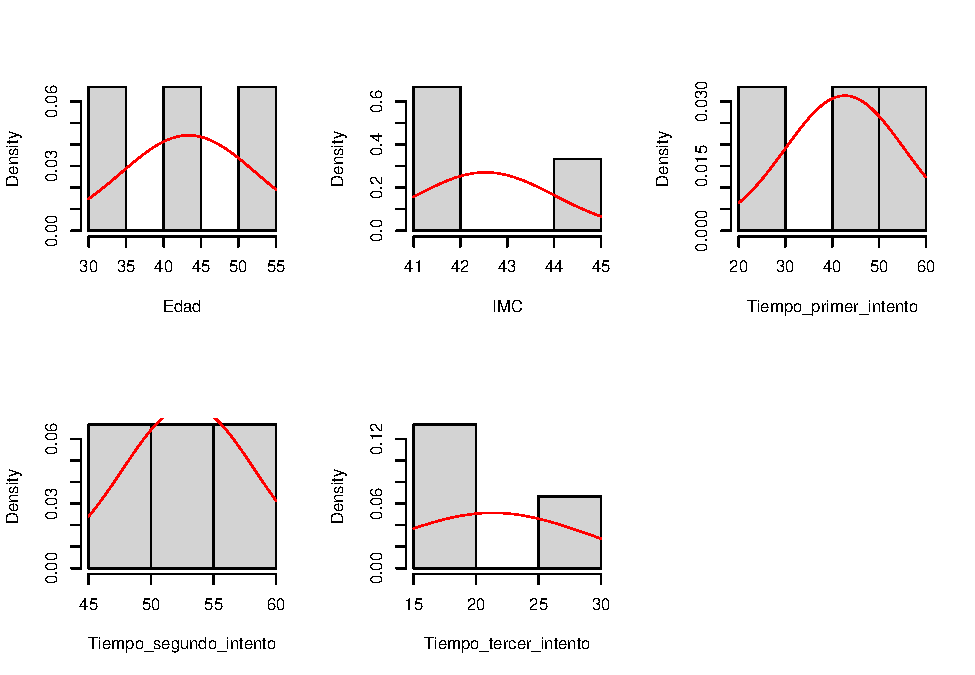
\includegraphics{Laringoscopia_files/figure-latex/unnamed-chunk-10-1.pdf}

\begin{Shaded}
\begin{Highlighting}[]
\NormalTok{m2}\SpecialCharTok{$}\NormalTok{univariateNormality}
\end{Highlighting}
\end{Shaded}

\begin{verbatim}
##           Test                Variable Statistic   p value Normality
## 1 Shapiro-Wilk      Num_Intentos          0.3462  <0.001      NO    
## 2 Shapiro-Wilk Tiempo_total_intubacion    0.8475  <0.001      NO    
## 3 Shapiro-Wilk    Nivel_dificultad        0.9240  <0.001      NO
\end{verbatim}

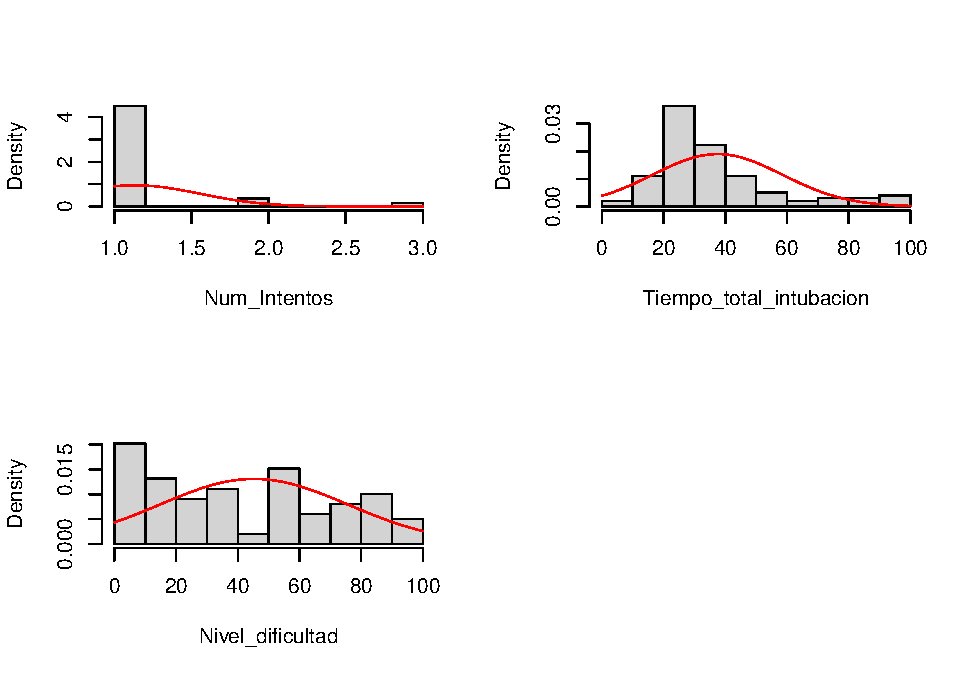
\includegraphics{Laringoscopia_files/figure-latex/unnamed-chunk-10-2.pdf}

\hypertarget{materiales-y-muxe9todos}{%
\section{Materiales y métodos}\label{materiales-y-muxe9todos}}

\hypertarget{anuxe1lisis-bivariado}{%
\subsection{Análisis bivariado}\label{anuxe1lisis-bivariado}}

\hypertarget{prueba-de-suma-de-rangos-de-wilcoxon-sin-ajuste-de-covariables-para-el-nuxfamero-de-intentos-de-intubaciuxf3n-y-tiempo-total-de-intubaciuxf3n}{%
\subsubsection{Prueba de suma de rangos de Wilcoxon (sin ajuste de
covariables) para el número de intentos de intubación y tiempo total de
intubación}\label{prueba-de-suma-de-rangos-de-wilcoxon-sin-ajuste-de-covariables-para-el-nuxfamero-de-intentos-de-intubaciuxf3n-y-tiempo-total-de-intubaciuxf3n}}

``La prueba de la U de Mann-Whitney, también denominada prueba de la
suma de rangos de Wilcoxon, es una prueba no paramétrica que permite
comparar las medianas de una variable cuantitativa para las dos
categorías de una variable cualitativa dicotómica. Se aplica cuando no
se pueden asumir los supuestos necesarios para utilizar la prueba de la
t de Student'' (2).

A diferencia de la prueba t de Student, la prueba U de Mann-Whitney
permite sacar diferentes conclusiones sobre los datos en función de las
suposiciones que se hagan sobre la distribución de los mismos.

Estas conclusiones pueden ir desde simplemente afirmar si las dos
poblaciones difieren hasta determinar si hay diferencias en las medianas
entre los grupos. Estas diferentes conclusiones dependen de la forma de
las distribuciones de los datos.

En este caso, como bien se menciona en el análisis estadístico del
artículo (3) uno de los principales objetivos

\begin{Shaded}
\begin{Highlighting}[]
\CommentTok{\# Extracción de columna de número de intentos de intubación por grupo}

\CommentTok{\# Número de intentos de intubación en grupo Macintosh}

\NormalTok{prueba\_Macintosh }\OtherTok{\textless{}{-}}\NormalTok{ datos }\SpecialCharTok{\%\textgreater{}\%}
                  \FunctionTok{filter}\NormalTok{(datos}\SpecialCharTok{$}\NormalTok{Grupo }\SpecialCharTok{==} \StringTok{"Macintosh"}\NormalTok{) }\SpecialCharTok{\%\textgreater{}\%}
                  \FunctionTok{select}\NormalTok{(Num\_Intentos, Tiempo\_total\_intubacion, Nivel\_dificultad, Mallampati, Sangrado, Dolor\_garganta)}

\CommentTok{\# Número de intentos de intubación en grupo Pentax\_AWS}

\NormalTok{prueba\_Pentax }\OtherTok{\textless{}{-}}\NormalTok{ datos }\SpecialCharTok{\%\textgreater{}\%}
               \FunctionTok{filter}\NormalTok{(datos}\SpecialCharTok{$}\NormalTok{Grupo }\SpecialCharTok{==} \StringTok{"Pentax\_AWS"}\NormalTok{) }\SpecialCharTok{\%\textgreater{}\%}
               \FunctionTok{select}\NormalTok{(Num\_Intentos, Tiempo\_total\_intubacion, Nivel\_dificultad, Mallampati, Sangrado, Dolor\_garganta)}
\end{Highlighting}
\end{Shaded}

\begin{Shaded}
\begin{Highlighting}[]
\CommentTok{\# Prueba de suma de rangos de Wilcoxon para el número de intentos de intubación}

\FunctionTok{wilcox.test}\NormalTok{(prueba\_Macintosh}\SpecialCharTok{$}\NormalTok{Num\_Intentos , prueba\_Pentax}\SpecialCharTok{$}\NormalTok{Num\_Intentos)}
\end{Highlighting}
\end{Shaded}

\begin{verbatim}
## 
##  Wilcoxon rank sum test with continuity correction
## 
## data:  prueba_Macintosh$Num_Intentos and prueba_Pentax$Num_Intentos
## W = 1172, p-value = 0.482
## alternative hypothesis: true location shift is not equal to 0
\end{verbatim}

La prueba arroja un valor p \textgreater{} α=0.05, por lo cual no se
puede rechazar \(H_0\), es decir, que no existe una diferencia
estadísticamente significativa entre el número de intentos de intubación
promedio del grupo Macintosh y Pentax AWS.

\begin{Shaded}
\begin{Highlighting}[]
\CommentTok{\# Prueba de suma de rangos de Wilcoxon}

\FunctionTok{wilcox.test}\NormalTok{ (prueba\_Macintosh}\SpecialCharTok{$}\NormalTok{Tiempo\_total\_intubacion, prueba\_Pentax}\SpecialCharTok{$}\NormalTok{Tiempo\_total\_intubacion)}
\end{Highlighting}
\end{Shaded}

\begin{verbatim}
## 
##  Wilcoxon rank sum test with continuity correction
## 
## data:  prueba_Macintosh$Tiempo_total_intubacion and prueba_Pentax$Tiempo_total_intubacion
## W = 489, p-value = 2.608e-07
## alternative hypothesis: true location shift is not equal to 0
\end{verbatim}

La prueba arroja un valor p \textless{} α=0.05, por lo cual se puede
rechazar \(H_0\), es decir, que existe una diferencia estadísticamente
significativa entre el tiempo de intubación total promedio del grupo
Macintosh y Pentax AWS.

\begin{Shaded}
\begin{Highlighting}[]
\CommentTok{\# Prueba de suma de rangos de Wilcoxon para el Nivel de dificultad de intubación}

\FunctionTok{wilcox.test}\NormalTok{(prueba\_Macintosh}\SpecialCharTok{$}\NormalTok{Nivel\_dificultad , prueba\_Pentax}\SpecialCharTok{$}\NormalTok{Nivel\_dificultad)}
\end{Highlighting}
\end{Shaded}

\begin{verbatim}
## 
##  Wilcoxon rank sum test with continuity correction
## 
## data:  prueba_Macintosh$Nivel_dificultad and prueba_Pentax$Nivel_dificultad
## W = 899, p-value = 0.02221
## alternative hypothesis: true location shift is not equal to 0
\end{verbatim}

\begin{Shaded}
\begin{Highlighting}[]
\CommentTok{\# Prueba de suma de rangos de Wilcoxon para la escala de Mallampati}

\FunctionTok{wilcox.test}\NormalTok{(prueba\_Macintosh}\SpecialCharTok{$}\NormalTok{Mallampati, prueba\_Pentax}\SpecialCharTok{$}\NormalTok{Mallampati)}
\end{Highlighting}
\end{Shaded}

\begin{verbatim}
## 
##  Wilcoxon rank sum test with continuity correction
## 
## data:  prueba_Macintosh$Mallampati and prueba_Pentax$Mallampati
## W = 1329.5, p-value = 0.3292
## alternative hypothesis: true location shift is not equal to 0
\end{verbatim}

\begin{Shaded}
\begin{Highlighting}[]
\CommentTok{\# Prueba de suma de rangos de Wilcoxon para sangrado }

\FunctionTok{wilcox.test}\NormalTok{(}\FunctionTok{as.numeric}\NormalTok{(prueba\_Macintosh}\SpecialCharTok{$}\NormalTok{Sangrado) , }\FunctionTok{as.numeric}\NormalTok{(prueba\_Pentax}\SpecialCharTok{$}\NormalTok{Sangrado))}
\end{Highlighting}
\end{Shaded}

\begin{verbatim}
## 
##  Wilcoxon rank sum test with continuity correction
## 
## data:  as.numeric(prueba_Macintosh$Sangrado) and as.numeric(prueba_Pentax$Sangrado)
## W = 1176, p-value = 0.1637
## alternative hypothesis: true location shift is not equal to 0
\end{verbatim}

\begin{Shaded}
\begin{Highlighting}[]
\CommentTok{\# Prueba de suma de rangos de Wilcoxon para sangrado }

\FunctionTok{wilcox.test}\NormalTok{(}\FunctionTok{as.numeric}\NormalTok{(prueba\_Macintosh}\SpecialCharTok{$}\NormalTok{Dolor\_garganta) , }\FunctionTok{as.numeric}\NormalTok{(prueba\_Pentax}\SpecialCharTok{$}\NormalTok{Dolor\_garganta))}
\end{Highlighting}
\end{Shaded}

\begin{verbatim}
## 
##  Wilcoxon rank sum test with continuity correction
## 
## data:  as.numeric(prueba_Macintosh$Dolor_garganta) and as.numeric(prueba_Pentax$Dolor_garganta)
## W = 1191.5, p-value = 0.9452
## alternative hypothesis: true location shift is not equal to 0
\end{verbatim}

\hypertarget{pruebas-de-asociaciuxf3n}{%
\subsection{Pruebas de asociación}\label{pruebas-de-asociaciuxf3n}}

\hypertarget{evaluaciuxf3n-del-efecto-de-tratamiento-sobre-las-variables-uxe9xito-de-intubaciuxf3n-en-el-primer-intento-uxe9xito-de-intubaciuxf3n-en-general-sagrando-y-visibilidad-de-la-glotis-mediante-la-prueba-exacta-de-fisher.}{%
\subsubsection{Evaluación del efecto de tratamiento sobre las variables:
éxito de intubación en el primer intento, éxito de intubación en
general, sagrando y visibilidad de la glotis, mediante la prueba exacta
de
Fisher.}\label{evaluaciuxf3n-del-efecto-de-tratamiento-sobre-las-variables-uxe9xito-de-intubaciuxf3n-en-el-primer-intento-uxe9xito-de-intubaciuxf3n-en-general-sagrando-y-visibilidad-de-la-glotis-mediante-la-prueba-exacta-de-fisher.}}

\begin{Shaded}
\begin{Highlighting}[]
\CommentTok{\# Creación de tablas de contingencia}

\CommentTok{\# Tratamiento vs éxito de intubación en el primer intento}

\NormalTok{t1 }\OtherTok{\textless{}{-}} \FunctionTok{table}\NormalTok{(datos}\SpecialCharTok{$}\NormalTok{Grupo, datos}\SpecialCharTok{$}\NormalTok{Exito\_primer\_intento)}

\CommentTok{\# Tratamiento vs éxito de intubación en general}

\NormalTok{t2 }\OtherTok{\textless{}{-}} \FunctionTok{table}\NormalTok{(datos}\SpecialCharTok{$}\NormalTok{Grupo, datos}\SpecialCharTok{$}\NormalTok{Exito\_intubacion)}

\CommentTok{\# Tratamiento vs sagrando}

\NormalTok{t3 }\OtherTok{\textless{}{-}} \FunctionTok{table}\NormalTok{(datos}\SpecialCharTok{$}\NormalTok{Grupo, datos}\SpecialCharTok{$}\NormalTok{Sangrado)}

\CommentTok{\# Tratamiento vs visibilidad de la glotis}

\NormalTok{t4 }\OtherTok{\textless{}{-}} \FunctionTok{table}\NormalTok{(datos}\SpecialCharTok{$}\NormalTok{Grupo, datos}\SpecialCharTok{$}\NormalTok{Vista\_glotis)}

\CommentTok{\# Tratamiento vs dolor de garganta}

\NormalTok{t5 }\OtherTok{\textless{}{-}} \FunctionTok{table}\NormalTok{(datos}\SpecialCharTok{$}\NormalTok{Grupo, datos}\SpecialCharTok{$}\NormalTok{Dolor\_garganta)}
\end{Highlighting}
\end{Shaded}

Odds ratio: measure of how far from independence the 2x2 table is H\_O:
odds ratio = 0 (no asociación) H\_a: odds ratio = 1 (asociación)

\begin{Shaded}
\begin{Highlighting}[]
\CommentTok{\# Prueba exacta e Fisher para tratamiento vs éxito de intubación en el primer intento}

\FunctionTok{fisher.test}\NormalTok{(t1)}
\end{Highlighting}
\end{Shaded}

\begin{verbatim}
## 
##  Fisher's Exact Test for Count Data
## 
## data:  t1
## p-value = 0.5246
## alternative hypothesis: true odds ratio is not equal to 1
## 95 percent confidence interval:
##  0.1098579 2.3436553
## sample estimates:
## odds ratio 
##  0.5493335
\end{verbatim}

Una vez realizada la prueba exacta de Fisher se tiene un valor p
\textgreater{} \(\alpha\) = 0.05, por lo cual no existe evidencia
estadística suficiente para rechazar (\(H_0\): No existe asociación
entre las variables), es decir, que el tratamiento no tiene un efecto
sobre el éxito de intubación en el primer intento.

\begin{Shaded}
\begin{Highlighting}[]
\CommentTok{\# Prueba exacta e Fisher para tratamiento vs éxito de intubación en general}

\FunctionTok{fisher.test}\NormalTok{(t2)}
\end{Highlighting}
\end{Shaded}

\begin{verbatim}
## 
##  Fisher's Exact Test for Count Data
## 
## data:  t2
## p-value = 0.1175
## alternative hypothesis: true odds ratio is not equal to 1
## 95 percent confidence interval:
##  0.000000 1.508182
## sample estimates:
## odds ratio 
##          0
\end{verbatim}

\begin{Shaded}
\begin{Highlighting}[]
\CommentTok{\# Prueba exacta e Fisher para tratamiento vs sagrando}

\FunctionTok{fisher.test}\NormalTok{(t3)}
\end{Highlighting}
\end{Shaded}

\begin{verbatim}
## 
##  Fisher's Exact Test for Count Data
## 
## data:  t3
## p-value = 0.4949
## alternative hypothesis: true odds ratio is not equal to 1
## 95 percent confidence interval:
##  0.1846149       Inf
## sample estimates:
## odds ratio 
##        Inf
\end{verbatim}

\begin{Shaded}
\begin{Highlighting}[]
\CommentTok{\# Prueba exacta e Fisher para tratamiento vs visibilidad de la glotis}

\FunctionTok{fisher.test}\NormalTok{(t4)}
\end{Highlighting}
\end{Shaded}

\begin{verbatim}
## 
##  Fisher's Exact Test for Count Data
## 
## data:  t4
## p-value = 0.308
## alternative hypothesis: true odds ratio is not equal to 1
## 95 percent confidence interval:
##  0.5596514 5.9612982
## sample estimates:
## odds ratio 
##   1.767874
\end{verbatim}

\begin{Shaded}
\begin{Highlighting}[]
\CommentTok{\# Prueba exacta e Fisher para tratamiento vs dolor de garganta}

\FunctionTok{fisher.test}\NormalTok{(t5)}
\end{Highlighting}
\end{Shaded}

\begin{verbatim}
## 
##  Fisher's Exact Test for Count Data
## 
## data:  t5
## p-value = 0.7382
## alternative hypothesis: two.sided
\end{verbatim}

\hypertarget{intervalos-de-confianza-a-95-para-la-proporciuxf3n-de-uxe9xito-de-intubaciuxf3n-en-el-primero-intento-y-uxe9xito-de-intubaciuxf3n-en-general}{%
\subsubsection{Intervalos de confianza a 95\% para la proporción de
éxito de intubación en el primero intento y éxito de intubación en
general}\label{intervalos-de-confianza-a-95-para-la-proporciuxf3n-de-uxe9xito-de-intubaciuxf3n-en-el-primero-intento-y-uxe9xito-de-intubaciuxf3n-en-general}}

\begin{Shaded}
\begin{Highlighting}[]
\CommentTok{\# Extracción de columna de éxito de intubación en el primer intento por grupo}

\CommentTok{\# Éxito de intubación en el primer intento en grupo Macintosh}

\NormalTok{Exito\_1int\_Macintosh }\OtherTok{\textless{}{-}}\NormalTok{ datos }\SpecialCharTok{\%\textgreater{}\%}
                  \FunctionTok{filter}\NormalTok{(datos}\SpecialCharTok{$}\NormalTok{Grupo }\SpecialCharTok{==} \StringTok{"Macintosh"}\NormalTok{) }\SpecialCharTok{\%\textgreater{}\%}
                  \FunctionTok{select}\NormalTok{(Exito\_primer\_intento)}

\CommentTok{\# Éxito de intubación en el primer intento en grupo Pentax\_AWS}

\NormalTok{Exito\_1int\_Pentax\_AWS }\OtherTok{\textless{}{-}}\NormalTok{ datos }\SpecialCharTok{\%\textgreater{}\%}
               \FunctionTok{filter}\NormalTok{(datos}\SpecialCharTok{$}\NormalTok{Grupo }\SpecialCharTok{==} \StringTok{"Pentax\_AWS"}\NormalTok{) }\SpecialCharTok{\%\textgreater{}\%}
               \FunctionTok{select}\NormalTok{(Exito\_primer\_intento)}
\end{Highlighting}
\end{Shaded}

\begin{Shaded}
\begin{Highlighting}[]
\CommentTok{\# Conteo de éxito de intubación en el primer intento para cada grupo}

\CommentTok{\# Conteo en grupo Macintosh}

\NormalTok{Exito\_1int\_Macintosh }\SpecialCharTok{\%\textgreater{}\%}  
  \FunctionTok{tabyl}\NormalTok{(Exito\_primer\_intento) }\SpecialCharTok{\%\textgreater{}\%} 
  \FunctionTok{adorn\_totals}\NormalTok{(}\StringTok{"row"}\NormalTok{)}
\end{Highlighting}
\end{Shaded}

\begin{verbatim}
##  Exito_primer_intento  n    percent
##                    No  4 0.08163265
##                    Si 45 0.91836735
##                 Total 49 1.00000000
\end{verbatim}

\begin{Shaded}
\begin{Highlighting}[]
\CommentTok{\# Conteo en grupo Pentax\_AWS}

\NormalTok{Exito\_1int\_Pentax\_AWS }\SpecialCharTok{\%\textgreater{}\%}  
  \FunctionTok{tabyl}\NormalTok{(Exito\_primer\_intento) }\SpecialCharTok{\%\textgreater{}\%} 
  \FunctionTok{adorn\_totals}\NormalTok{(}\StringTok{"row"}\NormalTok{)}
\end{Highlighting}
\end{Shaded}

\begin{verbatim}
##  Exito_primer_intento  n percent
##                    No  7    0.14
##                    Si 43    0.86
##                 Total 50    1.00
\end{verbatim}

\begin{Shaded}
\begin{Highlighting}[]
\CommentTok{\# Intervalos de confianza a 95\% para el éxito de intubación en el primer intento }
\CommentTok{\# Metodo Wilson (default)}

\CommentTok{\# Intervalo de confianza a 95\% para el éxito de intubación en el primer intento para grupo Macintosh}

\FunctionTok{BinomCI}\NormalTok{(}\DecValTok{45}\NormalTok{,}\DecValTok{49}\NormalTok{,}\AttributeTok{conf.level=}\FloatTok{0.95}\NormalTok{)}
\end{Highlighting}
\end{Shaded}

\begin{verbatim}
##            est    lwr.ci    upr.ci
## [1,] 0.9183673 0.8081087 0.9677972
\end{verbatim}

\begin{Shaded}
\begin{Highlighting}[]
\CommentTok{\# Intervalo de confianza a 95\% para el éxito de intubación en el primer intento para grupo Pentax\_AWS}

\FunctionTok{BinomCI}\NormalTok{(}\DecValTok{43}\NormalTok{,}\DecValTok{50}\NormalTok{,}\AttributeTok{conf.level=}\FloatTok{0.95}\NormalTok{)}
\end{Highlighting}
\end{Shaded}

\begin{verbatim}
##       est    lwr.ci    upr.ci
## [1,] 0.86 0.7381381 0.9304917
\end{verbatim}

\begin{Shaded}
\begin{Highlighting}[]
\CommentTok{\# Extracción de columna de éxito de intubación en general por grupo}

\CommentTok{\# Éxito de intubación en general en grupo Macintosh}

\NormalTok{Exito\_gen\_Macintosh }\OtherTok{\textless{}{-}}\NormalTok{ datos }\SpecialCharTok{\%\textgreater{}\%}
                  \FunctionTok{filter}\NormalTok{(datos}\SpecialCharTok{$}\NormalTok{Grupo }\SpecialCharTok{==} \StringTok{"Macintosh"}\NormalTok{) }\SpecialCharTok{\%\textgreater{}\%}
                  \FunctionTok{select}\NormalTok{(Exito\_intubacion)}

\CommentTok{\# Éxito de intubación en general en grupo Pentax\_AWS}

\NormalTok{Exito\_gen\_Pentax\_AWS }\OtherTok{\textless{}{-}}\NormalTok{ datos }\SpecialCharTok{\%\textgreater{}\%}
               \FunctionTok{filter}\NormalTok{(Grupo }\SpecialCharTok{==} \StringTok{"Pentax\_AWS"}\NormalTok{) }\SpecialCharTok{\%\textgreater{}\%}
               \FunctionTok{select}\NormalTok{(Exito\_intubacion)}
\end{Highlighting}
\end{Shaded}

\begin{Shaded}
\begin{Highlighting}[]
\CommentTok{\# Conteo de éxito de intubación en general para cada grupo}

\CommentTok{\# Conteo en grupo Macintosh}

\NormalTok{Exito\_gen\_Macintosh }\SpecialCharTok{\%\textgreater{}\%}  
  \FunctionTok{tabyl}\NormalTok{(Exito\_intubacion) }\SpecialCharTok{\%\textgreater{}\%} 
  \FunctionTok{adorn\_totals}\NormalTok{(}\StringTok{"row"}\NormalTok{)}
\end{Highlighting}
\end{Shaded}

\begin{verbatim}
##  Exito_intubacion  n percent
##                No  0       0
##                Si 49       1
##             Total 49       1
\end{verbatim}

\begin{Shaded}
\begin{Highlighting}[]
\CommentTok{\# Conteo en grupo Pentax\_AWS}

\NormalTok{Exito\_gen\_Pentax\_AWS }\SpecialCharTok{\%\textgreater{}\%} 
  \FunctionTok{tabyl}\NormalTok{(Exito\_intubacion) }\SpecialCharTok{\%\textgreater{}\%} 
  \FunctionTok{adorn\_totals}\NormalTok{(}\StringTok{"row"}\NormalTok{)}
\end{Highlighting}
\end{Shaded}

\begin{verbatim}
##  Exito_intubacion  n percent
##                No  4    0.08
##                Si 46    0.92
##             Total 50    1.00
\end{verbatim}

\begin{Shaded}
\begin{Highlighting}[]
\CommentTok{\# Intervalos de confianza a 95\% para el éxito de intubación en general}

\CommentTok{\# Intervalo de confianza a 95\% para el éxito de intubación en general para grupo Macintosh}

\FunctionTok{BinomCI}\NormalTok{(}\DecValTok{49}\NormalTok{,}\DecValTok{49}\NormalTok{,}\AttributeTok{conf.level=}\FloatTok{0.95}\NormalTok{)}
\end{Highlighting}
\end{Shaded}

\begin{verbatim}
##      est    lwr.ci upr.ci
## [1,]   1 0.9273022      1
\end{verbatim}

\begin{Shaded}
\begin{Highlighting}[]
\CommentTok{\# Intervalo de confianza a 95\% para el éxito de intubación en general para grupo Pentax\_AWS}

\FunctionTok{BinomCI}\NormalTok{(}\DecValTok{46}\NormalTok{,}\DecValTok{50}\NormalTok{,}\AttributeTok{conf.level=}\FloatTok{0.95}\NormalTok{)}
\end{Highlighting}
\end{Shaded}

\begin{verbatim}
##       est    lwr.ci    upr.ci
## [1,] 0.92 0.8116175 0.9684505
\end{verbatim}

\begin{Shaded}
\begin{Highlighting}[]
\CommentTok{\# 45 (resultado en el articulo)}
\end{Highlighting}
\end{Shaded}

\hypertarget{evaluaciuxf3n-del-efecto-de-pentax-en-el-nivel-de-dificultad-de-intubaciuxf3n-traqueal-y-severidad-de-dolor-en-la-garganta-postoperatorio-mediante-ancova}{%
\subsubsection{Evaluación del efecto de Pentax en el nivel de dificultad
de intubación traqueal y severidad de dolor en la garganta
postoperatorio mediante
ANCOVA}\label{evaluaciuxf3n-del-efecto-de-pentax-en-el-nivel-de-dificultad-de-intubaciuxf3n-traqueal-y-severidad-de-dolor-en-la-garganta-postoperatorio-mediante-ancova}}

\hypertarget{supuestos}{%
\paragraph{Supuestos}\label{supuestos}}

\hypertarget{linealidad}{%
\subparagraph{Linealidad}\label{linealidad}}

\begin{Shaded}
\begin{Highlighting}[]
\FunctionTok{ggplot}\NormalTok{(datos) }\SpecialCharTok{+}
  \FunctionTok{geom\_point}\NormalTok{( }\FunctionTok{aes}\NormalTok{(Nivel\_dificultad, Dolor\_garganta, }\AttributeTok{group=}\NormalTok{datos}\SpecialCharTok{$}\NormalTok{Grupo, }\AttributeTok{color=}\NormalTok{datos}\SpecialCharTok{$}\NormalTok{Grupo)) }\SpecialCharTok{+}
  \FunctionTok{facet\_wrap}\NormalTok{(datos}\SpecialCharTok{$}\NormalTok{Grupo)}
\end{Highlighting}
\end{Shaded}

\includegraphics{Laringoscopia_files/figure-latex/unnamed-chunk-30-1.pdf}

Al parecer no existe una relación lineal entre los puntos en ninguno de
los grupos, por lo tanto no se cumple el supuesto de linealidad. Sin
embargo dado que la finalidad del proyecto no es predecir \ldots{}

\begin{Shaded}
\begin{Highlighting}[]
\CommentTok{\#library(CatterPlots)}
\CommentTok{\#catplot(datos$Dolor\_garganta, datos$Nivel\_dificultad, tmpdat,}
\CommentTok{\#         xlab = "Dolor de garganta", ylab = "Nivel de dificultad de intubación")}
\end{Highlighting}
\end{Shaded}

\begin{Shaded}
\begin{Highlighting}[]
\NormalTok{Mean\_Dificultad }\OtherTok{\textless{}{-}} \FunctionTok{tapply}\NormalTok{(datos}\SpecialCharTok{$}\NormalTok{Nivel\_dificultad, datos}\SpecialCharTok{$}\NormalTok{Dolor\_garganta, mean)}
\FunctionTok{plot}\NormalTok{(Mean\_Dificultad)}
\end{Highlighting}
\end{Shaded}

\includegraphics{Laringoscopia_files/figure-latex/unnamed-chunk-32-1.pdf}

\hypertarget{homogeneidad-de-pendientes-de-regresiuxf3n}{%
\subparagraph{Homogeneidad de pendientes de
regresión}\label{homogeneidad-de-pendientes-de-regresiuxf3n}}

Esta prueba evalua si existe alguna interacción entre la covariable
(dolor de garganta) y el factor (grupo).

\begin{Shaded}
\begin{Highlighting}[]
\CommentTok{\# Ánalisis ANOVA}

\NormalTok{datos }\SpecialCharTok{\%\textgreater{}\%} \FunctionTok{anova\_test}\NormalTok{(Nivel\_dificultad }\SpecialCharTok{\textasciitilde{}}\NormalTok{ Grupo}\SpecialCharTok{*}\NormalTok{Dolor\_garganta)}
\end{Highlighting}
\end{Shaded}

\begin{verbatim}
## ANOVA Table (type II tests)
## 
##                 Effect DFn DFd     F     p p<.05   ges
## 1                Grupo   1  90 5.358 0.023     * 0.056
## 2       Dolor_garganta   3  90 1.761 0.160       0.055
## 3 Grupo:Dolor_garganta   3  90 0.528 0.664       0.017
\end{verbatim}

\begin{Shaded}
\begin{Highlighting}[]
\CommentTok{\# Existe un dato faltante en renglón 4 columna de dolor de garganta}
\CommentTok{\# ¿Se elimina?}

\NormalTok{datos[}\DecValTok{4}\NormalTok{,]}
\end{Highlighting}
\end{Shaded}

\begin{verbatim}
##   Edad   Genero Estado_fisico   IMC Mallampati     Grupo Tiempo_primer_intento
## 4   20 Femenino           III 46.32          2 Macintosh                    31
##   Exito_primer_intento Tiempo_segundo_intento Metodo_segundo_intento
## 4                   No                     46                     Si
##   Exito_segundo_intento Tiempo_tercer_intento Metodo_tercer_intento
## 4                    Si                    NA                  <NA>
##   Exito_tercer_intento Num_Intentos Fracasos Tiempo_total_intubacion
## 4                 <NA>            2        1                      77
##   Exito_intubacion Sangrado Nivel_dificultad Dolor_garganta Vista_glotis
## 4               Si       No               80           <NA>  Grado 1 o 2
##   Intentos_factor Mallampati_factor
## 4               2                II
\end{verbatim}

Se tiene un valor p mayor a 0.05 para la interacción entre la variable
grupo y la covariable dolor de gargante , por lo cual existe
homogeneidad de pendientes de regresión, es decir que sus pendientes de
regresión son paralelas.

\hypertarget{normalidad-en-residuales}{%
\subparagraph{Normalidad en residuales}\label{normalidad-en-residuales}}

\begin{Shaded}
\begin{Highlighting}[]
\FunctionTok{hist}\NormalTok{(datos}\SpecialCharTok{$}\NormalTok{Nivel\_dificultad)}
\end{Highlighting}
\end{Shaded}

\includegraphics{Laringoscopia_files/figure-latex/unnamed-chunk-34-1.pdf}

\begin{Shaded}
\begin{Highlighting}[]
\CommentTok{\# Fijar el modelo }

\NormalTok{model }\OtherTok{\textless{}{-}} \FunctionTok{lm}\NormalTok{(Nivel\_dificultad }\SpecialCharTok{\textasciitilde{}}\NormalTok{ Grupo, }\AttributeTok{data =}\NormalTok{ datos)}

\FunctionTok{summary}\NormalTok{(model)}
\end{Highlighting}
\end{Shaded}

\begin{verbatim}
## 
## Call:
## lm(formula = Nivel_dificultad ~ Grupo, data = datos)
## 
## Residuals:
##    Min     1Q Median     3Q    Max 
## -47.10 -27.65  -2.10  25.40  51.80 
## 
## Coefficients:
##                 Estimate Std. Error t value Pr(>|t|)    
## (Intercept)       38.204      4.258   8.971 2.23e-14 ***
## GrupoPentax_AWS   13.896      5.992   2.319   0.0225 *  
## ---
## Signif. codes:  0 '***' 0.001 '**' 0.01 '*' 0.05 '.' 0.1 ' ' 1
## 
## Residual standard error: 29.81 on 97 degrees of freedom
## Multiple R-squared:  0.05253,    Adjusted R-squared:  0.04276 
## F-statistic: 5.378 on 1 and 97 DF,  p-value: 0.02249
\end{verbatim}

\begin{Shaded}
\begin{Highlighting}[]
\CommentTok{\# Inspección del diagnóstico de métricas del modelo}

\NormalTok{model.metrics }\OtherTok{\textless{}{-}} \FunctionTok{augment}\NormalTok{(model)}

\CommentTok{\# Prueba de normalidad en los residuos usando shapiro wilk test}

\FunctionTok{shapiro\_test}\NormalTok{(model.metrics}\SpecialCharTok{$}\NormalTok{.resid)}
\end{Highlighting}
\end{Shaded}

\begin{verbatim}
## # A tibble: 1 x 3
##   variable             statistic   p.value
##   <chr>                    <dbl>     <dbl>
## 1 model.metrics$.resid     0.929 0.0000451
\end{verbatim}

Dado que se tiene un valor p \textless{} 0.05, existe evidencia
suficiente para rechazar \(h_0\), es decir, que los residuales no tienen
una aproximación a la normalidad.

\hypertarget{homogeneidad-de-varianzas}{%
\subparagraph{Homogeneidad de
varianzas}\label{homogeneidad-de-varianzas}}

\begin{Shaded}
\begin{Highlighting}[]
\CommentTok{\# Prueba de Levene}

\NormalTok{model.metrics }\SpecialCharTok{\%\textgreater{}\%} \FunctionTok{levene\_test}\NormalTok{(.resid }\SpecialCharTok{\textasciitilde{}}\NormalTok{ Grupo)}
\end{Highlighting}
\end{Shaded}

\begin{verbatim}
## # A tibble: 1 x 4
##     df1   df2 statistic     p
##   <int> <int>     <dbl> <dbl>
## 1     1    97      1.27 0.263
\end{verbatim}

La prueba de homogeneidad de varianzas de Levene arroja un valor p
\textgreater{} 0.05, lo que indica que no se puede rechazar \(H_0\), es
decir que existe homogeneidad entre las varianzas de los residuales de
cada grupo.

\hypertarget{valores-atuxedpicos}{%
\subparagraph{Valores atípicos}\label{valores-atuxedpicos}}

\begin{Shaded}
\begin{Highlighting}[]
\CommentTok{\# Verificación de valores atípicos}

\NormalTok{model.metrics }\SpecialCharTok{\%\textgreater{}\%} 
  \FunctionTok{filter}\NormalTok{(}\FunctionTok{abs}\NormalTok{(.std.resid) }\SpecialCharTok{\textgreater{}} \DecValTok{3}\NormalTok{) }\SpecialCharTok{\%\textgreater{}\%}   \CommentTok{\# Valor absoluto de .std.resid mayor a 3}
  \FunctionTok{as.data.frame}\NormalTok{()                  }
\end{Highlighting}
\end{Shaded}

\begin{verbatim}
## [1] Nivel_dificultad Grupo            .fitted          .resid          
## [5] .hat             .sigma           .cooksd          .std.resid      
## <0 rows> (or 0-length row.names)
\end{verbatim}

\hypertarget{ancova}{%
\paragraph{ANCOVA}\label{ancova}}

\begin{Shaded}
\begin{Highlighting}[]
\CommentTok{\#res.aov \textless{}{-} datos \%\textgreater{}\% }
 \CommentTok{\# anova\_test(datos$Nivel\_dificultad \textasciitilde{} datos$Dolor\_garganta + datos$Grupo)}
\end{Highlighting}
\end{Shaded}

\hypertarget{demografuxeda-y-evaluaciuxf3n-de-las-vuxedas-respiratorias}{%
\paragraph{Demografía y evaluación de las vías
respiratorias}\label{demografuxeda-y-evaluaciuxf3n-de-las-vuxedas-respiratorias}}

Datos

\begin{Shaded}
\begin{Highlighting}[]
\NormalTok{ttLCC }\OtherTok{\textless{}{-}}\NormalTok{ datos }\SpecialCharTok{\%\textgreater{}\%}
  \FunctionTok{group\_by}\NormalTok{(datos}\SpecialCharTok{$}\NormalTok{Grupo)}
  \FunctionTok{t.test}\NormalTok{(datos}\SpecialCharTok{$}\NormalTok{Edad,}\AttributeTok{conf.level =} \FloatTok{0.95}\NormalTok{)}
\end{Highlighting}
\end{Shaded}

\begin{verbatim}
## 
##  One Sample t-test
## 
## data:  datos$Edad
## t = 37.49, df = 98, p-value < 2.2e-16
## alternative hypothesis: true mean is not equal to 0
## 95 percent confidence interval:
##  46.80805 52.04044
## sample estimates:
## mean of x 
##  49.42424
\end{verbatim}

\begin{Shaded}
\begin{Highlighting}[]
\NormalTok{ttLCC}\SpecialCharTok{$}\NormalTok{estimate}
\end{Highlighting}
\end{Shaded}

\begin{verbatim}
## NULL
\end{verbatim}

\begin{Shaded}
\begin{Highlighting}[]
\NormalTok{df }\OtherTok{\textless{}{-}}\NormalTok{ datos }\SpecialCharTok{\%\textgreater{}\%}
  \FunctionTok{filter}\NormalTok{(datos}\SpecialCharTok{$}\NormalTok{Grupo }\SpecialCharTok{==} \StringTok{"Macintosh"}\NormalTok{) }

\NormalTok{df2 }\OtherTok{\textless{}{-}}\NormalTok{ datos }\SpecialCharTok{\%\textgreater{}\%}
  \FunctionTok{filter}\NormalTok{(datos}\SpecialCharTok{$}\NormalTok{Grupo }\SpecialCharTok{==} \StringTok{"Pentax\_AWS"}\NormalTok{) }
\end{Highlighting}
\end{Shaded}

\hypertarget{gruxe1ficas}{%
\section*{Gráficas}\label{gruxe1ficas}}
\addcontentsline{toc}{section}{Gráficas}

\hypertarget{refs}{}
\begin{CSLReferences}{0}{0}
\leavevmode\vadjust pre{\hypertarget{ref-curtosis}{}}%
\CSLLeftMargin{1. }%
\CSLRightInline{Sanjuán FJM. Curtosis. 2020; Available from:
\url{https://economipedia.com/definiciones/curtosis.html}}

\leavevmode\vadjust pre{\hypertarget{ref-Mann}{}}%
\CSLLeftMargin{2. }%
\CSLRightInline{Manuel M. Prueba de la u de mann-whitney. Ciencias o
letras. Available from:
\url{https://anestesiar.org/2022/prueba-de-la-u-de-mann-whitney-ciencias-o-letras/}}

\leavevmode\vadjust pre{\hypertarget{ref-Ab}{}}%
\CSLLeftMargin{3. }%
\CSLRightInline{Abdallah R, Galway U, You J, Kurz A, Sessler DI, Doyle
DJ. \href{https://doi.org/10.1213/ANE.0b013e31822cf47d}{A randomized
comparison between the pentax aws video laryngoscope and the macintosh
laryngoscope in morbidly obese patients}. Anesthesia and Analgesia.
2011;113:1082--7. }

\end{CSLReferences}

\end{document}
